%----------------------------------------------------------------
%
%  File    :  thesis-details.tex
%
%  Author  :  Keith Andrews, IICM, TU Graz, Austria
% 
%  Created :  17 Nov 2004
% 
%  Changed :  17 Nov 2004
% 
%----------------------------------------------------------------

\chapter{Selected Details of the Implementation
(and Test of Extremely
Long Chapter Titles to See How They Work or Not)
}

\label{chap:SelectedDetails}


\chapquote{
The devil is in the detail.
}
{
English proverb.
}


There are often specific details of a project, which involve
particularly much work to get right, but do not form a major part in
the whole scheme of things, so would not generally deserve a chapter
of their own. This chapter is for these details.



\section{First Selected Detail}

The context, the decision process, all the variations that were tried,
and the solution that was finally adopted.



\section{Second Selected Detail}

From some other part of the project. Explaining your reasoning and
choices will help some other poor student, who has to pick up your
work from where you left off.



\section{Using a Table}

An example of using a table can be seen in Table~\ref{tab:BestPubs}.

\begin{table}[tp]
\centering
\begin{tabularx}{\linewidth}{|llrX|}
\hline
Name & Type & Rating & Description \\
\hline
Flann O'Brien &
Irish &
***** &
In the centre of town and easy to find for
marauding tourists. Very smooth Guinness.
\\
\hline
The Office &
English &
***** &
Hidden in the narrow streets of the old town.
Erasmus student night every other Wednesday.
\\
\hline
O'Carolans &
Irish &
*** &
In the centre of town in a small side street next to Flann's.
Small, cosy, but hellishly smoky.
\\
\hline
O'Riginal &
pseudo Irish &
 &
Austrian dive pretending to be an Irish pub.
\\
\hline
\end{tabularx}

\caption[Best Pubs in Graz]
{
The best pubs in Graz.
}
\label{tab:BestPubs}
\end{table}





\section{Using Subfigures}

This example shows how to include vector graphics in the form of PDF
files. It also shows how to use subfigures within a figure.

\begin{figure}[tp]
\centering
\subfloat[][%  the % chars remove implicit spacing
An object has been composed to represent an
abstract version of the clock tower in Graz.
Here, the object is in its initial state.
]
{%
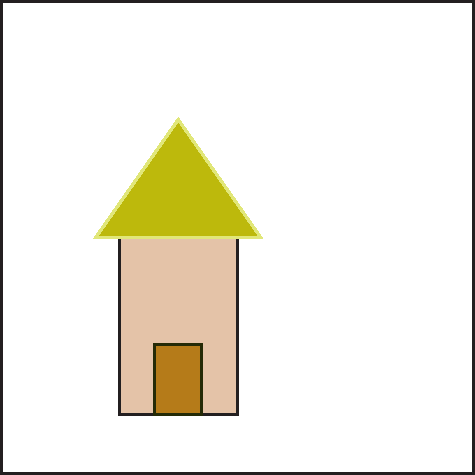
\includegraphics[width=0.45\linewidth]
{diagrams/multi1.pdf}%
\label{fig:Tower1}%
}
\hfill
\subfloat[][%
The object has been scaled and rotated, and now resembles
a leaning tower.
]
{%
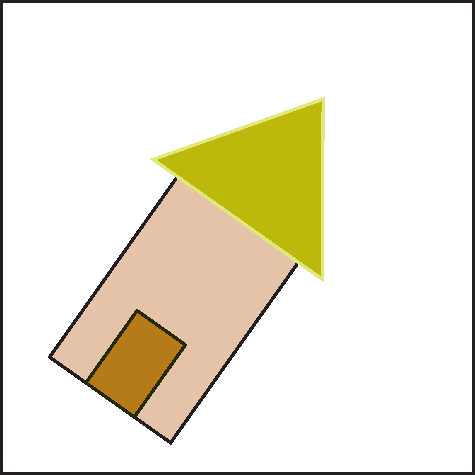
\includegraphics[width=0.45\linewidth]
{diagrams/multi2.pdf}%
\label{fig:Tower2}%
}

\caption[Abstract Clock Towers]
{
The leaning tower of Graz. An abstract model of the clock
tower in Graz leaning over time. \subref{fig:Tower1} shows
the initial state. \subref{fig:Tower2} shows the final state.
\imgcredit{Both images created by the author of this thesis.}
}
\label{fig:WholeFig}
\end{figure}


An example of using the \vname{subfig} package can be seen in
Figure~\ref{fig:WholeFig}. Figure~\ref{fig:Tower1} shows the polygons
before transformation, while Figure~\ref{fig:Tower2} shows them
afterwards.





\section{Including a Screenshot}

This example shows how to include a screenshot (or other raster
graphic) into a \LaTeXe\ figure.

\begin{figure}[tp]
\centering
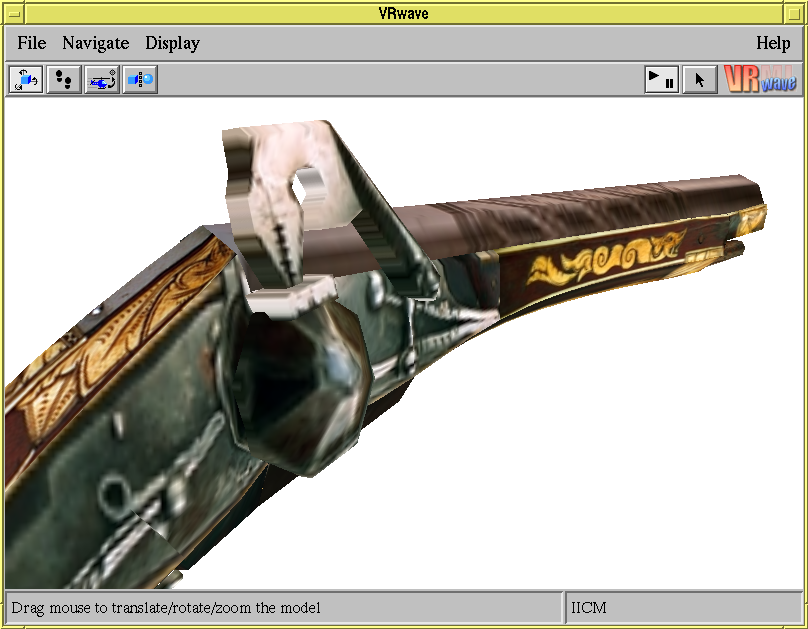
\includegraphics[keepaspectratio,width=\linewidth,height=\halfh]
{images/pist.png}

\caption[VRwave in Flip Mode]
{%
VRwave in Flip mode displaying a textured model of a cavalry pistol
from the world-renowned Zeughaus (armoury) in Graz.
\imgcredit{Image extracted from \textcite[page~81]{Andrews-VRwave}
and used under the terms of the ACM Copyright Policy. \copyrightACM}
}
\label{fig:Pistol}
\end{figure}


An example of how to correctly cite the source when using an image
from someone else. In their 1998 paper, \textcite{Andrews-VRwave}
discuss the VRwave VRML browser. Figure~\ref{fig:Pistol} shows a VRML
model of a cavalry pistol from the Armoury in Graz displayed in the
VRwave VRML browser.





\section{Using Special Characters and Symbols}

You can use many (but not all) of the thousands of characters
available in the UTF-8 \parencites{Wikipedia-UTF8}{Unicode-Charts}
character encoding. For example, the German umlauts (äüö), the German
sharp s (ß), or the yen symbol (¥).

You can also try some of the \approxsym 100 symbols available
in the \vname{textcomp} package, such as the yen symbol (\textyen) and
a circled letter A (\textcircled{A}).



\section{Using Macros to Style Special Names}

Use the \vname{vname}, \vname{cname}, and \vname{fname} macros to
define the style for (say) variable names, class names, and file
names. You can also define your own macros. The is a very long file
name \fname{/usr/data/keith/travel/austria/vienna.txt} to see how they
are broken at a line end. A typical class name is
\cname{HVSInformationPyramidsInputFactory}.





\section{Using Macros as Shorthand}

Sometimes, a macro (new command definition) can be useful to define
the contents of table cells, particularly if these contain images. For
example, Table~\ref{tab:WinIconicLang} uses the macro called
\vname{iibox}, which takes a single parameter, the name of
the particular image.


\begin{table}[tp]

\newcommand{\iibox}[1]{\parbox[c][1cm][c]{1cm}{%
\includegraphics[scale=0.6]{./images/icons/#1.png}
}}

\begin{center}
\begin{tabular}[t]{|p{7cm}c|}
\hline
\multicolumn{2}{|l|}{\sffamily \bfseries Elementary Symbols}            \\
Document                            & \iibox{win-il-gen-doc}            \\
Assistant                           & \iibox{win-il-gen-ass}            \\
Template                            & \iibox{win-il-gen-tmpl}           \\
\hline
\multicolumn{2}{|l|}{\sffamily \bfseries Document Types}                \\
Text document                       & \iibox{win-il-text-doc}           \\
Spreadsheet document                & \iibox{win-il-spreadsheet-doc}    \\
Presentation document               & \iibox{win-il-presentation-doc}   \\
Database document                   & \iibox{win-il-database-doc}       \\
\hline
\multicolumn{2}{|l|}{\sffamily \bfseries Applications}                  \\
Word                                & \iibox{win-il-word-appl}          \\
Excel                               & \iibox{win-il-xls-appl}           \\
Powerpoint                          & \iibox{win-il-ppt-appl}           \\
Access                              & \iibox{win-il-mdb-appl}           \\
\hline
\multicolumn{2}{|l|}{\sffamily \bfseries Generated Icons}               \\
Word text document                  & \iibox{win-il-word-doc}           \\
Excel spreadsheet document          & \iibox{win-il-xls-doc}            \\
Powerpoint presentation document    & \iibox{win-il-ppt-doc}            \\
Access database document            & \iibox{win-il-mdb-doc}            \\[2ex]
%
Word template                       & \iibox{win-il-word-tmpl}          \\
Powerpoint template                 & \iibox{win-il-ppt-tmpl}           \\
Access template                     & \iibox{win-il-mdb-tmpl}           \\[2ex]
%
Word template assistant             & \iibox{win-il-word-ass}           \\
Powerpoint template assistant       & \iibox{win-il-ppt-ass}            \\
Access template assistant           & \iibox{win-il-mdb-ass}            \\[2ex]
%
\hline
\end{tabular}
\end{center}

\caption[Iconic language for Windows NT 4.0 documents]
{
Iconic language for Windows NT 4.0 documents.
\imgcredit{The icons are screenshots, captured and then
enlarged by the author of this thesis.}
}
\label{tab:WinIconicLang}
\end{table}







\begin{samepage}
\begin{lstlisting}[%
  float=tp,
  aboveskip=\floatsep,
  belowskip=\floatsep,
  xleftmargin=0cm,              % no extra margins for floats
  xrightmargin=0cm,             % no extra margins for floats
  basicstyle=\footnotesize\ttfamily,
  frame=shadowbox,
  numbers=left,
  language=HTML,
  label=list:HTML5Boilerplate,
  caption={[HTML5 Boilerplate Code]%
Some HTML5 boilerplate code, illustrating the typical structure
of a HTML5 web page.
},
]
<!DOCTYPE html>
<html xmlns="http://www.w3.org/1999/xhtml" lang="en" xml:lang="en">

<head>
<meta charset="UTF-8"/>
<meta name="viewport" content="width=device-width, initial-scale=1"/>
<link rel="stylesheet" href="./inm.css"/>

<title>Keith Andrews Web Page</title>
</head>

<body>

<header>
<img src="images/kalogo.svg" alt="KA Logo"/>
Keith Andrews Design
</header>

<h1>Keith Andrews</h1>

<p>
Keith lives in <a href="http://graz.at/">Graz</a>.
</p>

<p>
<img src="images/keith-s.jpg"
  alt="Photo of Keith Andrews"/>
</p>

<p>
Three desirable attributes:
</p>
<ol>
<li>cheap</li>
<li>fast</li>
<li>good</li>
</ol>
<p>
Choose any two.
</p>

<p>
<abbr title="Extensible HyperText Markup Language">XHTML</abbr>
is cool.
</p>

<table>
<tbody>
<tr><th>Beer</th><th>Price €</th></tr>
<tr><td>Puntigamer</td><td>2,60</td></tr>
<tr><td>Gösser</td><td>2,60</td></tr>
<tr><td>Guinness</td><td>4,35</td></tr>
</tbody>
</table>

<footer>
Copyright © Keith Andrews 2019.
</footer>

</body>
</html>
\end{lstlisting}
\end{samepage}



\section{Using Floating Listings}

Listing~\ref{list:HTML5Boilerplate} is floating. A floating listing is
a block of code treated like other \LaTeXe floats (such as figures or
tables). Use floating listings for longer blocks of code.
A floating listing is given a number and can be referred to
explicitly, like Listing~\ref{list:HTML5Boilerplate}. It can be given
a caption and short caption, and is listed in the List of Listings.





\section{Using Non-Floating Diplayed Listings}

The listing below shows some CSS:
\begin{samepage}
\begin{lstlisting}[%
  language=CSS,
]
body { color: black; background-color: silver; }
img { border: none; }
h1,h2 { font-family: Verdana, sans-serif; }
\end{lstlisting}
\end{samepage}
It is displayed (i.e. indented as a block) in-place, but is not
floating. It cannot be referred to by number and is not listed in the
List of Listings. As a rule of thumb, if listings have five or more
lines, make them floating.





\section{Using Inline Listings}

Inline listings are used for very short snippets of code embedded
within the flow of a paragraph. For example,
\lstinline|\lstinline!var i:integer;!|
produces
\lstinline!var i:integer;!, which can now be discussed further.
Do not break an inline listing over multiple lines (EOL).




\section{Using Lists}

A list should always be introduced by a sentence
which ends with a colon.
%
There are three kinds of standard lists in \LaTeXe:
\begin{itemize}
\item itemize
\item enumerate
\item description
\end{itemize}
% A blank line here would indicate a new (indented) paragraph
An enumerated list has numbered items:
\begin{enumerate}
\item Fast
\item Good
\item Cheap
\end{enumerate}
Choose any two!


A description list has named items with corresponding
definitions or descriptions:
\begin{description}
\item[Short] Each item has a label (name) and its description.

\item[Rather longer label] By default, if the description text
  is rather long, it will warp around to the following lines.
\end{description}



